\chapter{How congestion shapes cities}
\label{chap:monocentric_model}

\begin{flushright}{\slshape    
What is here required is a new kind of statistical mechanics,\\
in which we renounce exact knowledge not\\
of the state of the system but\\
of the nature of the system itself.}  \\ \medskip
--- Freeman J. Dyson~\cite{Dyson:1962}
\end{flushright}


\bigskip


We saw in chapter~\ref{chap:monocentric_introduction} that as cities grow and
expand, they evolve from a monocentric organisation where all the activities are
concentrated in the same geographical area -- usually the central business
district -- to a more distributed, polycentric organisation. In this chapter, we
will try to uncover the mechanisms at play behind this transition. We begin with
a brief introduction of the model of Fujita and Ogawa in urban economics. We
will highlight the issues of this model, before presenting our model. This model
is a stochastic, out-of-equilibrium model and relies on the assumption that the
polycentric structure of large cities might find its origin in congestion,
irrespective of the particular local economic details. We are able to reproduce
many stylized facts, and -- most importantly -- to derive a general relation
between the number of activity centers of a city and its population. 


\section{Fujita and Ogawa}
\label{sec:fujita_and_ogawa}

In line with the tradition of economic geography~\cite{Fujita:2001}, the model
of Fujita and Ogawa~\cite{Fujita:1982} is based on the concept of agglomeration
economies---to explain why economical activities tend to group---and the spatial
distribution of wages and rents across the urban space. They consider that
cities are constituted of two kinds of actors: the firms, who tend to
concentrate to maximise their production, and the households, who try to
minimise their rent and commuting cost.\\ 

The model is \emph{static}, in the sense that the numbers of firms and
individuals are fixed. It is an \emph{equilibrium} model, and considers that the
city is the realisation of a general optimum. The original model is also
\emph{one-dimensional}, although the hypothesis of one-dimensionality is not
fundamental, and only necessary to make the calculations easier. Because we 
do not try to solve the model, we write equations in the more general
two-dimensional case.

\subsection{Households} 
\label{sub:households}

Fujita and Ogawa assume that there is a fixed number $N$ of households in the
city. The households are considered identical, in the sense that they all have
the same utility function and the same budget constraint. The utility function
of each household is given by the function $U = U(Z)$ where $Z$ is the surplus
of money that is left after budgetary constraints (expressed in monetary units);
basically, the money one has left at the end of the month, once the rent, bills
and petrol (or transportation card) have been paid. 

The utility is assumed to be an increasing function of $Z$ so

\begin{equation}
    \frac{\partial U}{\partial Z} > 0
\end{equation}

The budget constraint on an household living at $i$ (of coordinates $\vec{x}$)
and working at the firm located at $j$ (of coordinates $\vec{y}$) is given by the
equation

\begin{equation}
    Z = W\left(j\right)
      - C_R\left(i\right)
      - C_T\left(i,j\right)
\end{equation} 

where $W\left(j\right)$ is the wage earned at $j$, $C_R\left(i\right)$ the total
rent paid at $i$ and $C_T\left(i,j\right)$ the cost of commuting between
home and work. This equation is very general, and will be our starting point for
the model presented in the next section. The authors of~\cite{Fujita:1982}
further specify the commuting cost

\begin{equation}
    C_T\left(i,j\right) = t\,d_E(i,j) = t\,\left|\vec{y}-\vec{x}\right|
\end{equation}

where $t$ represents the commuting cost per unit distance, and $d_E(i,j) = \left| \vec{y} -
\vec{x} \right|$ the euclidean distance between home and work. The total rent
cost is further written as

\begin{equation}
    C_R\left(i\right) = R(i)\,S_h
\end{equation}

where $R(i)$ is the rent per unit surface at $i$, and $S_h$ the surface area
used by households, which becomes a parameter of the model.  The surplus $Z$
thus finally reads

\begin{equation}
    Z = W\left(j\right)
      - R\left(i\right)\,S_h
      - t\,d_E\left(i,j\right)
\end{equation} 


\subsection{Firms}
\label{sub:firms}

The second type of agents taken into consideration in the model are the firms.
It is assumed that all firms employ the same number of individuals, which
amounts to having a fixed number $M$ of firms (once the number of households is
fixed). The profit earned by a firm  located at $j$ reads, in a general
form

\begin{equation}
    \Pi = G\left(j\right) 
        - C_R\left(j\right) 
        -  W\left(j\right)\,L_f
\end{equation}

where $G(j)$ is the total gain realised by the firm selling its production,
$C_R(j)$ the rent paid by the firm, and $L_f$ the total number of employees per
firm---a parameter of the model.\\

To take agglomeration economies into account, Fujita and Ogawa define the
locational potential $F$ defined by

\begin{equation}
    F\left(j\right) = \int_{\mathcal{C}} b(\vec{x})\,e^{-\alpha\,\left|\vec{y}-\vec{x}\right|}\:\mathrm{d}\vec{x}
\end{equation}

where $b(\vec{x})$ is the density of firms at $\vec{x}$. The integral runs over
the entire city's spatial extent $\mathcal{C}$. One can easily see that the
higher the density of firms in a radius of $1/\alpha$ around a firm, the higher
the locational potential is going to be. Balanced by the constraint imposed by
the rent, which prevents too many firms from agglomerating at the same location,
the locational potential likely is the term responsible for the existence of
polycentric solutions in the model. Indeed, the authors further write the total
gain $G$ as a multiple of $F$:

\begin{equation}
    G(j) = \beta\,F(j)
\end{equation}

where $\beta$ integrates both the productivity of the employees and the effect
of the locational potential. The rent, as
in the case of households, is written $C_R(j) = R(j)\,S_f$ where $S_f$, the
surface needed by firms, is a parameter of the model. The profit
of companies therefore reads

\begin{equation}
    \Pi = \beta\, \int_{\mathcal{C}} b(\vec{x})\,e^{-\alpha\,\left|\vec{y}-\vec{x}\right|}\:\mathrm{d}\vec{x}
        - R\left(j\right)\,S_f
        - W\left(j\right)
\end{equation}


\subsection{Equilibrium conditions and results}
\label{sub:equilibrium_conditions}

Once the budget constraints have been explicited, one needs to define
the equilibrium conditions to be able to solve the model. First, the goal of
each household is to maximise their utility under the budget constraint. That
is, to choose $Z$, $S$, $\vec{x}$ and $\vec{y}$ so that $U(S,Z)$ is maximum.

Here, the maximisation of utility under budget constraints is
equivalent to chosing the residential location $i$ and the job location $j$ so
as to maximise $Z$. In other words, the maximisation of utility in this
particular situation is equivalent to performing a cost-benefit analysis.\\ 

The firms have no utility function, and choose to be a the location $j$ that
maximises their profit.\\

A further constraint is given by the bid-rent curve, and determines the spatial
interaction between households and firms. The authors define two intermediate
functions, $\Psi(\vec{x})$ and $\Phi(\vec{x})$ which are respectively the bid
rent function of households and of firms, defined as

\begin{align}
    \Psi\left(\vec{x}\right) &= \max_{\vec{x}} \left\{ \frac{1}{S_h} \left[W(\vec{x} ) - Z -
    t\,d_E\left(\vec{x}-\vec{y}\right)\right] | U(Z) = U\right\}\\
    \Phi\left(\vec{x}\right) &= \frac{1}{S_f} \left[\beta\,F(\vec{y}) - \Pi -
W(\vec{y})\right]
\end{align}

$\Psi(\vec{x})$ represents the maximum rent that the households could pay to be
located at $\vec{x}$ while still having a utility value $U$. $\Phi(\vec{y})$ is
the maximum rent that firms could pay to be located at $\vec{y}$. At
equilibrium, it is assumed that whoever's bid rent function has the highest
value at $\vec{x}$ will be located at $\vec{x}$.

Taken together, the equilibrium conditions determine the spatial distribution of
households and firms, of the wages and land prices.\\

The results of this model, given its intricacy, are somewhat disappointing.
Unsurprisingly, the authors are not able to derive an analytical solution for
their model. What they do, however, is deriving the conditions on the parameters
for the existence of monocentric and polycentric organisations of activities,
using numerical methods.

\section{Problems with the Fujita and Ogawa model}
\label{sec:problems_with_the_fujita_and_ogawa_model}

The approach of Fujita \& Ogawa fails at giving a satisfactory quantitative account  of the
polycentric transition of cities. A lot can be said about the details of the
model and its assumptions. But we choose to only discuss the issues that we
feel are the most important, and that we will try to address in our model. 

\paragraph{It is an equilibrium model.} In line with the rest of Urban
Economics~\cite{Fujita:2001, Fujita:2013}, the authors describe a city as being in
an equilibrium characterised by static spatial distributions of households and
business firms. However, the equilibrium assumption is unsupported as cities are
out-of-equilibrium systems and their dynamics is of particular interest for
practical applications~\cite{Batty:2008}.

\paragraph{It is too complex.} The model integrates so many interactions and
variables that it is difficult to understand the hierarchy of processes
governing the evolution of cities: which ones are fundamental and which ones are
irrelevant. A model is however only interesting when it provides a simple
structure to understand empirical results, whether it reproduces them, or
provides well-understood limiting cases (`null models').

\paragraph{It does not make any prediction.} Worse, due to its complexity, the
model is unsolvable, and does not make any prediction. At best it shows that
polycentric configurations are \emph{possible}. Yet, there are possibly
different models that would admit polycentric activity profiles as a solution.
The constraint is not strong enough, the model is unsupported by data.\\ 

We also note that the model does not take congestion into account in the
commuting cost (which is only a function of the distance). However, as we saw in
Chapter~\ref{chap:monocentric_introduction}, it is
mentioned in the economics literature as being a possible cause of the
polycentric transition of cities~\cite{McMillen:2003}. 


\section{Modeling mobility patterns}
\label{sec:an_out_of_equilibrium_model_}

In this section, we start from the model by Fujita \& Ogawa to propose a
dynamical model of city growth. Following recent interdisciplinary efforts to
construct a quantitative description of cities and their
evolution~\cite{Makse:1995,Zanette:1997,Marsili:1998,Bettencourt:2007,Batty:2008},
we deliberately omit certain details and focus instead on basic processes. We
thereby aim at building a minimal model which captures the complexity of the
system and is able to account for -- qualitative as well as quantitive -- stylized
facts.  

The model we propose is by essence dynamical and describes the evolution
of cities' organisation as their population increases. We focus on car
congestion -- mainly due to journey-to-work commutes -- and its effect on the
job location choice for individuals.\\

\subsection{Decoupling the choice of household location and job}
\label{sub:decoupling_the_choice_of_household_and_job}

The time scales involved in the evolution of cities are usually such that the
employment turnover rate is larger than the relocation rate of households. On a
short time scale, we can thus focus on the process of job-seeking alone, leaving
aside the problem of the choice of residence. In other words, we assume the
coupling between both processes to be negligible: we assume that each inhabitant
newly added to the city has a random residence location and we concentrate on
understanding how such an inhabitant chooses its job location.\\

As a result of this assumption, a worker living at $i$
will choose to work at the center $j$ such that the quantity
 
\begin{equation}
    Z_{ij} = W(j) - C_T(i,j)
    \label{eq:Z_workers_general}
\end{equation}

is maximum. Doing so, we give up any hope to describe the spatial structure of the rent
distribution, or the alledged scaling between rent prices and population size in
cities~\cite{Bettencourt:2013}.

\subsection{Decoupling the behaviour of firms and individuals}
\label{sub:decoupling_the_dynamics_of_}

Another difficulty with the Fujita-Ogawa model is the strong coupling between
the behaviour of firms and individuals. The empirical literature on the
behaviour of firms points to a tendency of similar industries to cluster
geographically~\cite{Duranton:2005, Marcon:2009}, and a higher
profit of industries located in Urban environments~\cite{Melo:2009}. Although
theoretical attempts at explaining these behaviours have been
proposed~\cite{Duranton:2004}, the models are yet to be developped in an
out-of-equilibrium framework.\\

Here, we decide to simplify the problem by assuming that firms indeed cluster
into specific locations, that we call activity centers. Each worker can then
choose among a pool of $N_c$ potential activity centers (whose locations are
randomly distributed across the city). The active subcenters are then
defined as the subset of potential centers which have a non zero incoming number
of individuals. We thus assume that the existence of activity centers is defined
by the willingness of workers to work in the possible locations.\\


Let us now discuss the form of the wage $W(j)$ and the commuting cost $C_T(i,j)$ that are
present in equation~\ref{eq:Z_workers_general}. 

\subsection{Determining the wage}
\label{sub:determining_the_wage}

The problem of determining the (spatial) variations of the average wage $W(j)$
at location $j$ is very reminiscent of some problems encountered in fundamental
physics. Indeed, the wage depends on many different factors, ranging from the
type of company, the education level of the inhabitant, the level of
aglomeration, etc., and in this respect is not too different from quantities
that can be measured in a large atom made of a large number of interacting
particles. In this situation, physicists figured that although it is possible
to write down the corresponding equations, not only is it impossible to solve
them, but also not really useful. In fact they found out that
a statistical description of these systems, relying on random matrices could
lead to predictions which agree with experimental results~\cite{Dyson:1962}.\\

We wish to import in spatial economics this idea of replacing a complex quantity
such as wages -- which depends on so many factors and interactions -- by a random
one. The problem is not so much that we cannot write down the equations that
determine the wage that an individual could get in a given company. Even if we
could (and we can't), the sheer number of people living in an urban area would prevent us
from solving these equations. And even if we could solve them, the resulting
information would be too overwhelming to really allow us to \emph{understand} the
behaviour of the system as a whole. We thus need an \emph{effective}
description of the phenomemon.

We account for the interaction between activity centers and
people by taking the wage in location $j$ as proportional to a random variable
$\eta_j \in \left[ 0,1\right]$ such that $W(j) = s\, \eta_j$ where $s$ defines
the maximum attainable average wage in the considered city.\\

We are aware that wages are not determined endogeneously but are instead the
result of thousands, millions of interactions between firms and individuals. In
the same way that Dyson did not mean that the interactions between electrons in
large atoms \emph{are} random, our assumptions does not mean that wages are
\emph{really} randomly determined. What we mean, however, is that in the case of
systems containing a large number of individuals, one may do \emph{as
if they were randomly determined}. Although we thereby abandon the possibility
to describe the dynamics of the wages and their spatial distribution, the
resulting model is analytically solvable and makes quantitative predictions.

\subsection{Commuting cost and congestion}
\label{sub:the_commuting_cost}


We choose the transportation cost $C_T(i,j)$ proportional to the commuting time
between $i$ and $j$. In a typical situation where passenger transportation is
dominated by personal vehicles, this commuting time not only depends on the
distance between $i$ and $j$, but also on the traffic between the two places,
the vehicle capacity of the underlying network and its resilience to congestion.
The Bureau of Public Road formula~\cite{Branston:1976} proposes a simple form
taking all these ingredients into account. In our framework, it leads to the
following expression for the commuting costs

\begin{equation}
    C_T(i,j) =  t\, d_{ij} \left[ 1 + \left( \frac{T_{ij}}{c} \right)^{\mu} \right]
    \label{eq:commuting_cost}
\end{equation}

where $T_{ij}$ the trafic per unit of time between $i$ and $j$ and $c$
is the typical capacity of a road (taken constant here). The quantity
$\mu$ is a parameter quantifying the resilience of the transportation
network to congestion. We further simplify the problem by assuming
than the traffic $T_{ij}$ is only a function of the subcenter $j$ and
therefore write $T_{ij}=T(j)$ the total traffic incoming in subcenter
$j$.

\subsection{Summary}
\label{sub:summary}


In summary, our model is defined as follows. At each time step, we add
a new individual $i$ located at random in the city, who will
choose to work in the activity area $j$ (among $N_c$ possibilities
located at random) such that the following quantity

\begin{equation}
    Z_{ij} = \eta_j - \frac{d_{ij}}{\ell} \left[ 1 + \left( \frac{T(j)}{c} \right)^{\mu} \right]
    \label{eq:cost_function}
\end{equation}

is maximum (we omitted irrelevant multiplicative factors). The quantity $\ell =
s/t$ is interpreted as the maximum effective commuting distance that people can
financially withstand. Interestingly, the presence of commuting costs entails the
existence of a second length scale $\ell$ in the system (the first one being the
typical size $L$ of the city).

\section{Monocentric to polycentric transition}
\label{sub:monocentric_to_polycentric_transition}

Depending on the relative importance of wages, distance and congestion, the
model predicts the existence of three different regimes: the monocentric regime
(Top left Figure~\ref{fig:model_results}), the distance-driven polycentric (Top
right Figure~\ref{fig:model_results}) regime and the attractivity-driven
polycentric (Bottom Figure~\ref{fig:model_results}) regime.\\


\begin{figure}
    \centering
    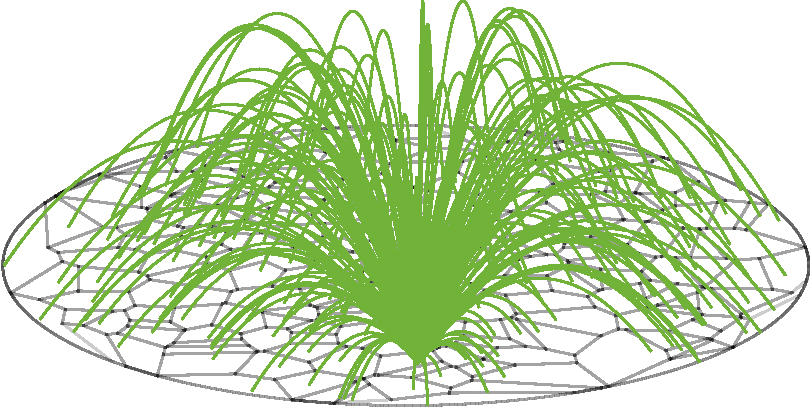
\includegraphics[width=0.49\textwidth]{gfx/chapter-monocentric/1.pdf}
    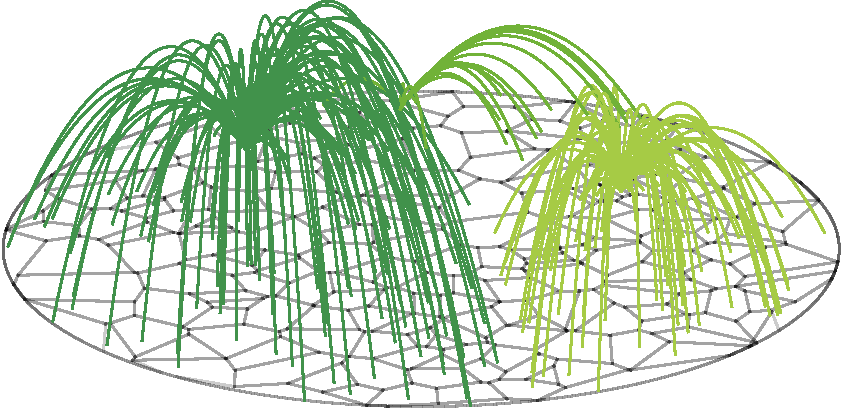
\includegraphics[width=0.49\textwidth]{gfx/chapter-monocentric/2.pdf}
    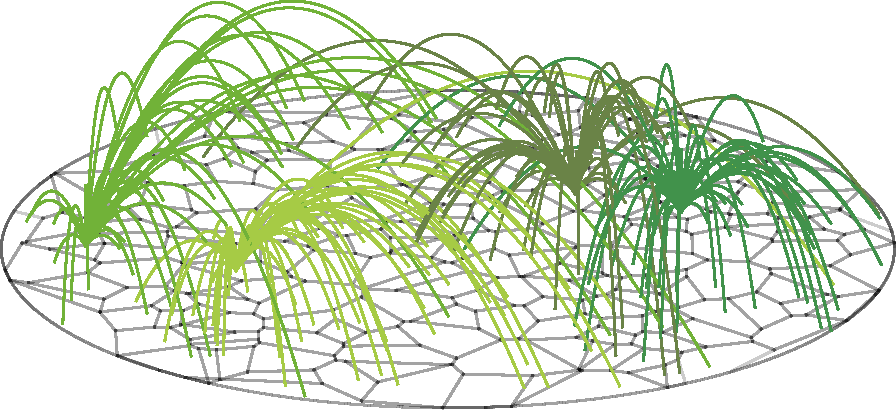
\includegraphics[width=0.49\textwidth]{gfx/chapter-monocentric/3.pdf}
    \caption{{\bf The different regimes.} The monocentric (top left), distance-driven polycentric (top right)
      and attractivity-driven polycentric (bottom) regimes as produced by
      our model. Each link represents a commuting journey to an activity center. \label{fig:model_results}}
\end{figure}

The existence of a monocentric regime depends on how $\ell$ -- the maximum
commuting distance that people can afford -- compares to the size of the city
$L$. Indeed, people located at a distance $d > \ell$ from the most
attractive center will not be able to afford commuting to this center, and will,
according to our model, choose to commute to a closer center.  As a result, a
monocentric regime is only sustainable as long as people's residence is drawn
close to the most attractive center. Thus, in the limit where $\ell \ll L$, the
attractiveness of a center becomes irrelevant, and a monocentric regime cannot
exist. In this case, we end up in the situation shown on the top-right of
Figure~\ref{fig:model_results}.\\


From now on, we will assume that $\ell$ is large enough so that a
monocentric state exists for small values of the population. In this
regime, the value of $\eta$ prevails and the monocentric state evolves
to an attractivity-driven polycentric structure as the population
increases. 
Starting from a small city with a monocentric
organisation, the traffic is negligible and 

$$Z_{ij}\approx \eta_j$$

which implies that all individuals are going to choose the most attractive
center, with the largest value of $\eta_j$, say $\eta_1$.
When the number $P$ of individuals increases, the traffic will also increase and
some initially less attractive centers (with a smaller values of $\eta$) might
become more attractive, leading to the appearance of a new subcenter. More specifically, a new
subcenter $j$ will appear when for an individual $i$, we have 

$$Z_{ij}>Z_{i1}$$

Because we assumed we originally were in a monocentric state, the traffic at
this point is such that $T(1)=P$ and $T(j)=0$ which leads to the equation

\begin{equation}
    \eta_j-\frac{d_{ij}}{\ell}>\eta_1-\frac{d_{i1}}{\ell}\left[1+\left(\frac{P}{c}\right)^\mu\right]
\end{equation}

We assume that there are no spatial correlations in the subcenter distribution,
so that we can make the approximation $d_{ij}\sim d_{i1}\sim L$. The new
subcenter will thus be such that $\eta_1-\eta_j$ is minimum. It will thus be the
potential subcenter with the second largest value denoted by $\eta_j=\eta_2$.\\

According to order statistics, we have on average for a uniform distribution

$$\overline{\eta_1-\eta_2}\simeq 1/N_c$$

hence a critical value for the population

\begin{equation}
    \boxed{P^*= c \left( \frac{\ell}{L N_c} \right)^{1/\mu}}
    \label{eq:critical_population}
\end{equation}

Whatever the system considered, there will \emph{always} be a critical
value of the population above which the city becomes polycentric. The
monocentric regime is therefore fundamentally unstable with regards to
population increase, which is in agreement with the fact that no major city in
the world exhibits a monocentric structure. We note that the smaller the value
of $\mu$ (or larger the value of the capacity $c$), the larger the critical
population value $P^*$ which means that cities with a good road system capable
of absorbing large traffic should display a monocentric structure for a longer
period of time.

\section{Number of centers}
\label{sec:number_of_centers}


We have so far established that, because of increased levels of congestion as
the population grows, all cities will eventually adopt a polycentric
structure. Although appealing and in agreement with common observations, the
prediction given by Eq.~\ref{eq:critical_population} is impossible to test with
the currently available data. Therefore, we would like to obtain a prediction
for the variation of the number of subcenters with population.\\

We compute the value of the population at which 
the $k^{th}$ center appears. Still in the attractivity-driven regime, we assume
that so far $k-1$
centers have emerged with 

$$\eta_{1} \geq \eta_{2} \geq \ldots \geq \eta_{k-1}$$

with a number of commuters $T(1), T(2), \ldots,
T(k-1)$, respectively. The next worker $i$ will choose the center $k$ if

\begin{equation}
    Z_{ik} > \max_{j \in \left[1,k-1\right]} Z_{ij}
\end{equation}

which reads

\begin{equation}
    \eta_k - \frac{d_{ik}}{\ell} > \max_{j \in \left[1,k-1\right]} \left\{
    \eta_j - \frac{d_{ij}}{\ell} \left[ 1 + \left(
      \frac{T(j)}{c}\right)^\mu\right] \right\}
\end{equation}

According to simulations of the model, we know that the distribution of traffic $T(j)$ is
narrow~\cite{Louf:2013_polycentric}, and we can assume that all the centers have roughly the same number of
commuters $T(j) \sim P/(k-1)$. As above we also assume that there are no spatial
correlations in the position of employment centers so that $d_{ij} \sim d_{ik} \sim L$. 
We can now write the previous expression as


\begin{equation}
\frac{L}{\ell} \left( \frac{P}{(k-1)\,c} \right)^{\mu} > \max_{j \in
  \left[1,k-1\right]} \left( \eta_j \right) - \eta_k
\end{equation}

Following our definitions, $\max_{j \in \left[1,k-1\right]} \left( \eta_j
\right) = \eta_1$. According to order statistics, if the $\eta_j$ are uniformly
distributed, we have on average $$\overline{\eta_1 - \eta_k} = (k-1)/(N_c+1)$$ 

It follows from these assumptions that (1) the $k^{th}$ center to appear is the
$k^{th}$ most attractive one (2) the average value of the population
$\overline{P}_k$ at which the $k^{th}$ center appears is given by:

\begin{equation} 
    \overline{P}_k = P^* \left( k-1 \right)^{\frac{\mu+1}{\mu}}
\end{equation}

Conversely, the number $k$ of subcenters scales sublinearly with population size as

\begin{equation} 
    \boxed{k \sim \left( \frac{P}{P^*} \right)^{\frac{\mu}{\mu
    + 1}}}
    \label{eq:centers_prediction}
\end{equation} 

For positive values of $\mu$, we have $\frac{\mu}{\mu+1}<1$. we can thus
conclude that the number of activity subcenters in urban areas scales sublinearly
with their population where the prefactor and the exponent depend on the
properties of the transportation network of the city under consideration. This
prediction is in agreement with the scalings obtained for Spanish and American
cities in Chapter~\ref{chap:monocentric_introduction}.



\section{Conclusion}
\label{sec:conclusion}

\subsection{A predictive model}
\label{sub:a_predictive_mode}

The model we just presented, although not perfect, exhibits many of the
desirable features of a model we listed in the introduction. First, it goes
beyond the standard models in urban economics by going beyond the explanation of
simple, qualitative, stylized facts. As we saw earlier, one major problem with the model of Fujita
and Ogawa is the absence of quantitative prediction. Instead of providing a
prediction that can be further confirmed or refuted by empirical observation,
the authors merely test the existence of polycentric solutions in the
framework of their model. The link with reality is however very loose, in the
sense that there is a big intellectual leap between the actual prediction of the
model and reality. Even though the model proposed here is very simple, it is not
difficult to link it to reality. Once the notion of activity centers is defined
empirically, it is not difficult to count the number of centers and look at the
dependence of this number on the population size of cities. The
model can then be confirmed, or refuted. Furthermore, as we will see in the
following section, the model serves as a basis to the understanding of some of
the scaling relationships in cities, linking the model even more strongly to 
empirical reality.

\subsection{Understanding the polycentric transition}
\label{sub:understanding_the_polycentric_tranistion}

Second, the model allows us to \emph{understand} why the polycentric transition
occurs. Taking a step back on the assumptions that lead to the prediction of
Eq.~\ref{eq:centers_prediction}, one can see that the transition
in our model is triggered by the congestion term in Eq.~\ref{eq:cost_function}. The positions
of households and firms are indeed taken as random, the wages are also taken at
random. Therefore, we can conclude that our model explains the polycentric
transition of cities through the increasing congestion around employment centers
as the population increase. More mechanisms are probably involved, but the model
shows that congestion alone is enough to lead to a polycentric situation.\\

If we assume that agglomeration economies is the basic process explaining the
existence of centers in the first place, the model provides evidence that this
centripetal force is balanced by the centrifugal effect of congestion that
tears city apart. Arguably, the non trivial spatial patterns observed in large cities can
 be understood as a result of the interplay between these competing
processes.\\

The model we propose trades off exhaustivity and complexity for simplicity and
explanatory power. Although some of the hypothesis we made are debatable, it is
striking that we manage to make a prediction on the scaling of the number of
centers with population size. On the other hand, unlike simplistic model, our
model's ontology is hard-wired into the reality we experience. For this reason,
its assumptions can be discussed, possibly changed. The model can be improved
upon in many different ways.
